The reference \ac{nse} achieved with the optimized parameter set from Assignment~1 is 0.908. The local \ac{sa} perturbs each of the 18 \acp{mp} individually between $-30\%$ and $+30\%$ of its calibrated value in 120 steps, with the objective function evaluated at each step. The results are organized below following the structure of the HBV001a model: the overall ranking, the sensitivity scatter plots for each module, the simulated discharge response for selected parameters, and the internal model state diagnostics.

\vspace{0.5cm}
\noindent\textbf{Overall parameter ranking}

Figure~\ref{fig:ranking_MP} ranks all 18 \acp{mp} by the maximum absolute relative change in \ac{ofv} observed across the full $\pm 30\%$ perturbation range. The ranking immediately shows that only a small subset of parameters controls model performance, while the majority are effectively inactive within the calibrated configuration.

\begin{figure}[!ht]
\centering
  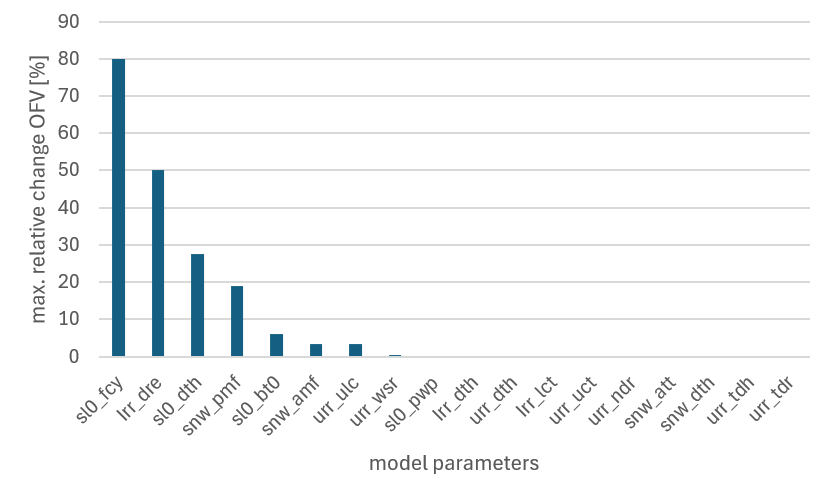
\includegraphics[width=0.88\textwidth]{Figures/Ass_02/new/ranking_localSA.png}
    \caption{Ranking of all 18 \acp{mp} by maximum absolute relative \ac{ofv} change within the $\pm 30\%$ perturbation range. Higher bars indicate stronger influence on model performance.}
    \label{fig:ranking_MP}
\end{figure}

Assuming that the optimized parameter set represents the global optimum from Assignment~1, any perturbation is expected to degrade or leave unchanged the \ac{ofv}. The results are largely consistent with this expectation. Three \acp{mp} show a marginal \ac{nse} improvement of at most 0.015, attributable to the finite resolution of the Differential Evolution optimizer near a flat objective surface.

\vspace{0.5cm}
\noindent\textbf{Sensitivity scatter plots by HBV module}

The following figures show, for each \ac{mp}, the relative change in the \ac{ofv} as a function of the relative perturbation applied to that parameter. A steep or wide scatter indicates a sensitive parameter; a flat, near-zero response indicates insensitivity. We also analyze which parameters hit their physical boundaries during the $\pm 30\%$ perturbation based on the boundary check results.

\vspace{0.3cm}
\noindent\textbf{Snow module (\texttt{snw\_*})}

Figure~\ref{fig:scatter_snw_1} and figure~\ref{fig:scatter_snw_2} display the scatter plots for the snow module. The most sensitive parameters within the snow module are the melt factors. \ref{fig:hbv_sl0fcy} shows that the high flow event is influenced by snow melt, and due to the short calibration time, this event has a main influence on the \ac{nse}. Thus, a sensitivity concerning snow parameters was expected. 
The calibrated \texttt{snw\_dth} value of 0.0 means the parameter is already at its absolute lower bound, so any perturbation percentage relative to 0.0 results in 0.0, keeping it clamped. 

\begin{figure}[!ht]
    \centering
    \begin{minipage}[t]{0.45\textwidth}
        \centering
        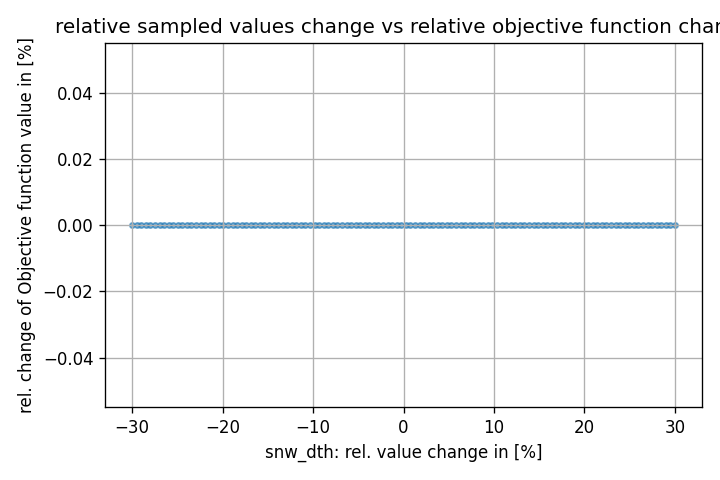
\includegraphics[width=\textwidth]{Figures/Ass_02/new/param_scatter_snw_dth.png}
    \end{minipage}
    \hfill
    \begin{minipage}[t]{0.45\textwidth}
        \centering
        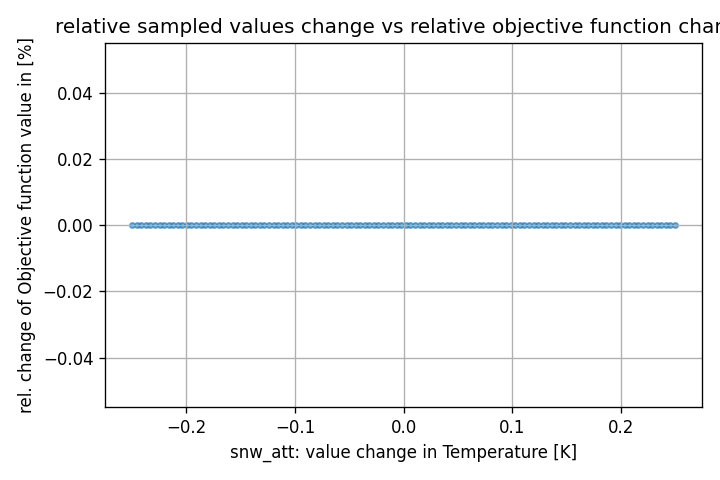
\includegraphics[width=\textwidth]{Figures/Ass_02/new/param_scatter_snw_att.png}
    \end{minipage}
    \caption{Sensitivity scatter plots for \texttt{snw\_dth} (initial snow depth) and \texttt{snw\_att} (melt–freeze threshold).}
    \label{fig:scatter_snw_1}
\end{figure}

\begin{figure}[!ht]
    \centering
    \begin{minipage}[t]{0.45\textwidth}
        \centering
        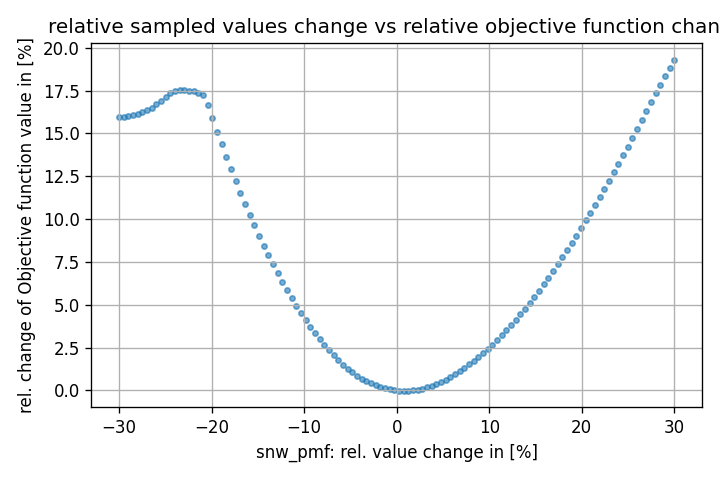
\includegraphics[width=\textwidth]{Figures/Ass_02/new/param_scatter_snw_pmf.png}
    \end{minipage}
    \hfill
    \begin{minipage}[t]{0.45\textwidth}
        \centering
        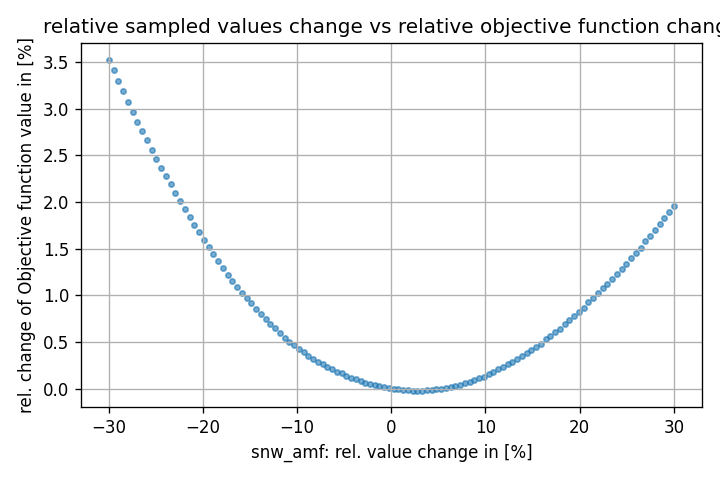
\includegraphics[width=\textwidth]{Figures/Ass_02/new/param_scatter_snw_amf.png}
    \end{minipage}
    \caption{Sensitivity scatter plots for \texttt{snw\_pmf} (precipitation melt factor) and \texttt{snw\_amf} (air temperature melt factor).}
    \label{fig:scatter_snw_2}
\end{figure}

\vspace{0.3cm}
\noindent\textbf{Soil module (\texttt{sl0\_*})}

Figure~\ref{fig:scatter_sl0_1} and figure~\ref{fig:scatter_sl0_2} show the soil module parameters, which contain two of the most sensitive parameters in the entire model. \texttt{sl0\_dth} and \texttt{sl0\_pwp} show a strongly asymmetric response: positive perturbations rapidly push the parameter toward its absolute upper bound, drastically reducing the soil's buffering capacity. Negative perturbations cause a more continuous \ac{nse} change. Using different optimization sets of \ac{mp} has shown that when sensitive parameters are constrained by boundaries, this alters the ranking of \ac{mp} sensitivity slightly (fig: \ref{fig:ranking_MP}).

\begin{figure}[!ht]
    \centering
    \begin{minipage}[t]{0.45\textwidth}
        \centering
        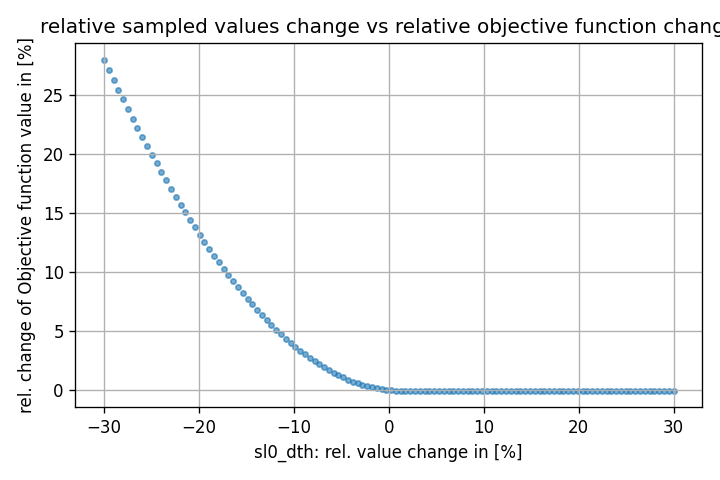
\includegraphics[width=\textwidth]{Figures/Ass_02/new/param_scatter_sl0_dth.png}
    \end{minipage}
    \hfill
    \begin{minipage}[t]{0.45\textwidth}
        \centering
        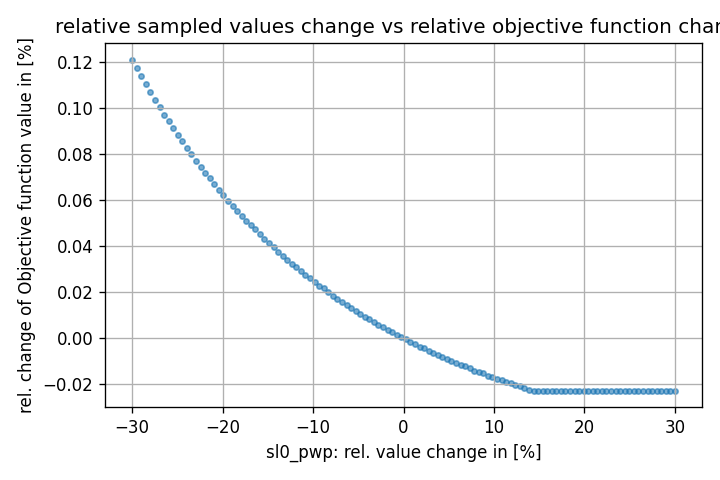
\includegraphics[width=\textwidth]{Figures/Ass_02/new/param_scatter_sl0_pwp.png}
    \end{minipage}
    \caption{Sensitivity scatter plots for \texttt{sl0\_dth} (initial soil depth) and \texttt{sl0\_pwp} (permanent wilting point).}
    \label{fig:scatter_sl0_1}
\end{figure}

\begin{figure}[!ht]
    \centering
    \begin{minipage}[t]{0.45\textwidth}
        \centering
        
\includegraphics[width=\textwidth]{Figures/Ass_02/new/param_scatter_sl0_fcy.png}
    \end{minipage}
    \hfill
    \begin{minipage}[t]{0.45\textwidth}
        \centering
        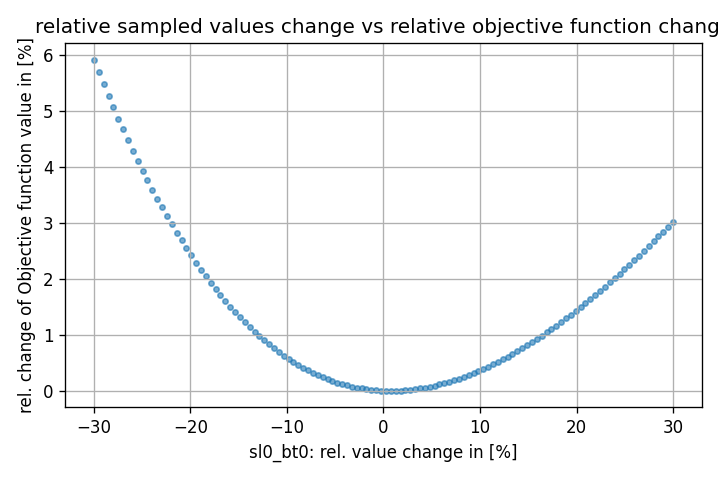
\includegraphics[width=\textwidth]{Figures/Ass_02/new/param_scatter_sl0_bt0.png}
    \end{minipage}
    \caption{Sensitivity scatter plots for \texttt{sl0\_fcy} (field capacity) and \texttt{sl0\_bt0} (beta exponent).}
    \label{fig:scatter_sl0_2}
\end{figure}

\vspace{0.3cm}
\noindent\textbf{Upper reservoir (\texttt{urr\_*})}

Figures~\ref{fig:scatter_urr_1} through \ref{fig:scatter_urr_4} show the seven upper reservoir parameters. \texttt{urr\_ulc} is the most influential among them. It regulates the percolation rate to the lower reservoir, which has the most influence on the discharge \ref{fig:hbv_sl0fcy}. This was also already discovered during the turnoff processes in assignment 1. \texttt{urr\_wsr} calibrated value of 0.997 is already near the upper bound of 1.0, so positive perturbations above $+22.9\%$ are clamped to 1.0, producing a flat response. The other parameters (\texttt{urr\_dth}, \texttt{urr\_uct}, \texttt{urr\_ndr}, \texttt{urr\_tdh}, \texttt{urr\_tdr}) show negligible sensitivity.

\begin{figure}[!ht]
    \centering
    \begin{minipage}[t]{0.45\textwidth}
        \centering
        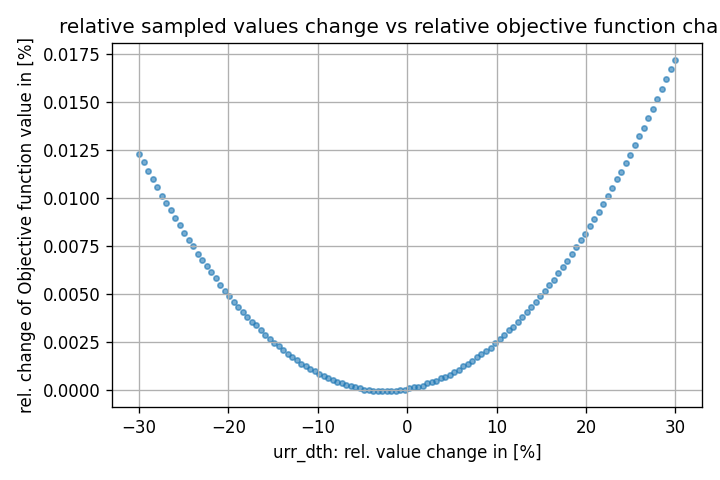
\includegraphics[width=\textwidth]{Figures/Ass_02/new/param_scatter_urr_dth.png}
    \end{minipage}
    \hfill
    \begin{minipage}[t]{0.45\textwidth}
        \centering
        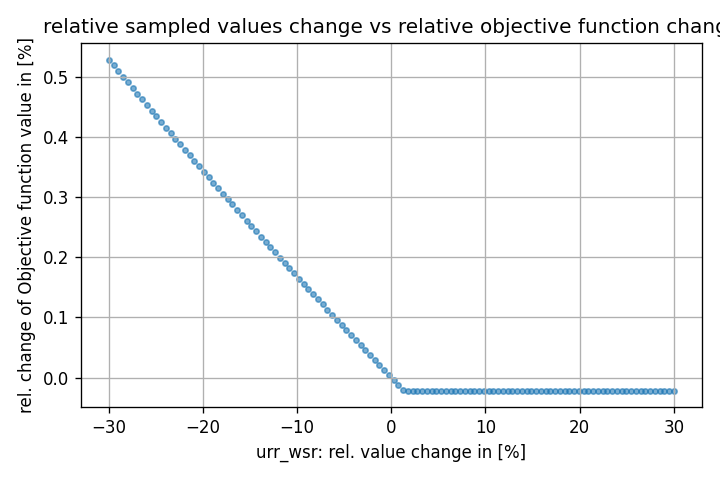
\includegraphics[width=\textwidth]{Figures/Ass_02/new/param_scatter_urr_wsr.png}
    \end{minipage}
    \caption{Sensitivity scatter plots for \texttt{urr\_dth} and \texttt{urr\_wsr} (water split ratio).}
    \label{fig:scatter_urr_1}
\end{figure}

\begin{figure}[!ht]
    \centering
    \begin{minipage}[t]{0.45\textwidth}
        \centering
        
\includegraphics[width=\textwidth]{Figures/Ass_02/new/param_scatter_urr_ulc.png}
    \end{minipage}
    \hfill
    \begin{minipage}[t]{0.45\textwidth}
        \centering
        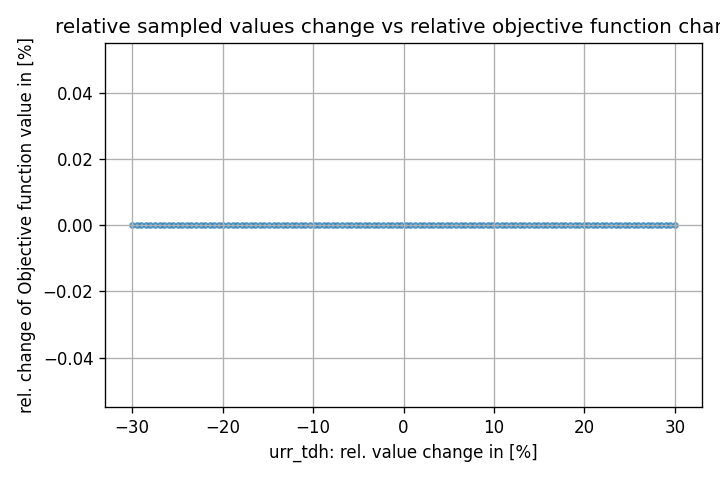
\includegraphics[width=\textwidth]{Figures/Ass_02/new/param_scatter_urr_tdh.png}
    \end{minipage}
    \caption{Sensitivity scatter plots for \texttt{urr\_ulc} and \texttt{urr\_tdh}.}
    \label{fig:scatter_urr_2}
\end{figure}

\begin{figure}[!ht]
    \centering
    \begin{minipage}[t]{0.45\textwidth}
        \centering
        
\includegraphics[width=\textwidth]{Figures/Ass_02/new/param_scatter_urr_tdr.png}
    \end{minipage}
    \hfill
    \begin{minipage}[t]{0.45\textwidth}
        \centering
        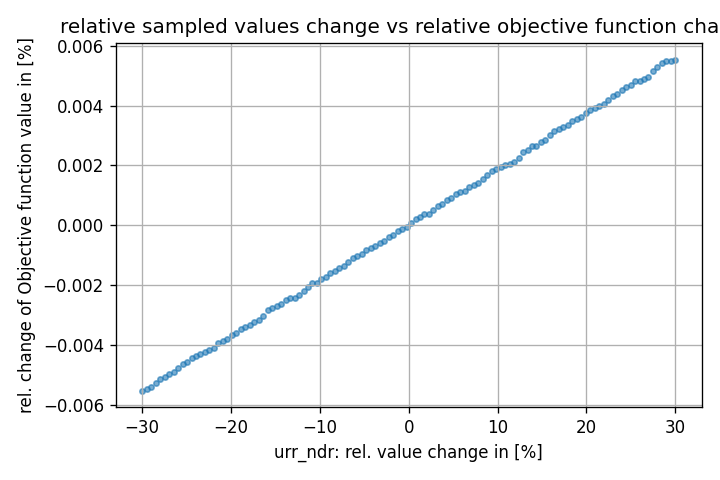
\includegraphics[width=\textwidth]{Figures/Ass_02/new/param_scatter_urr_ndr.png}
    \end{minipage}
    \caption{Sensitivity scatter plots for \texttt{urr\_tdr} and \texttt{urr\_ndr}.}
    \label{fig:scatter_urr_3}
\end{figure}

\begin{figure}[!ht]
    \centering
    \begin{minipage}[t]{0.45\textwidth}
        \centering
        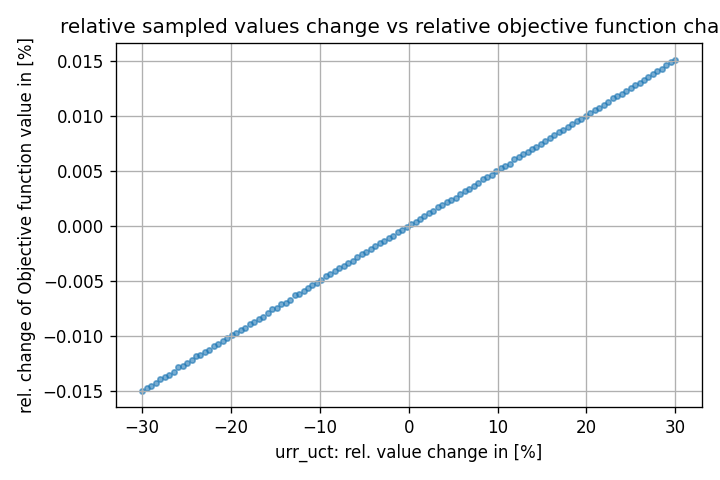
\includegraphics[width=\textwidth]{Figures/Ass_02/new/param_scatter_urr_uct.png}
    \end{minipage}
    \caption{Sensitivity scatter plot for \texttt{urr\_uct}.}
    \label{fig:scatter_urr_4}
\end{figure}

\vspace{0.3cm}
\noindent\textbf{Lower reservoir (\texttt{lrr\_*})}

Finally, figure~\ref{fig:scatter_lrr_1} and figure~\ref{fig:scatter_lrr_2} show the lower reservoir parameters. With \texttt{lrr\_dre} being one of the most sensitive parameters, as a ratio of the slow responding outflow, which is the main driver in this model for the discharge. \texttt{lrr\_lct} show near-zero sensitivity. This is consistent with expectations: the slow baseflow leaving the catchment without entering the river, governed by the lower reservoir, is a relatively minor fraction of the water balance during the short duration. None of these parameters hit boundary constraints.

\begin{figure}[!ht]
    \centering
    \begin{minipage}[t]{0.45\textwidth}
        \centering
        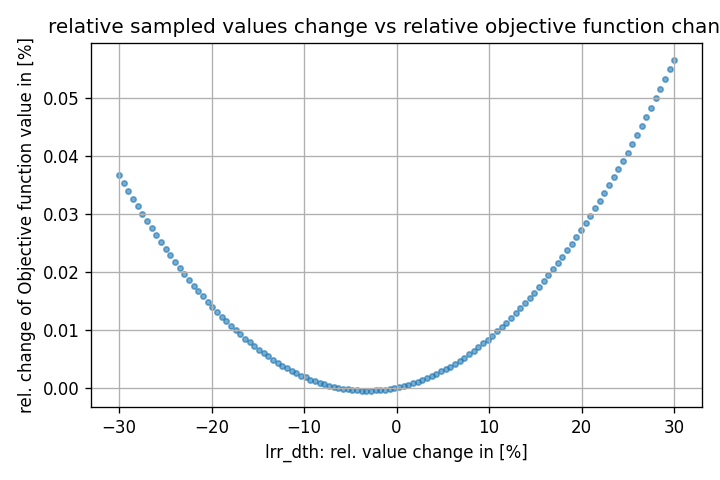
\includegraphics[width=\textwidth]{Figures/Ass_02/new/param_scatter_lrr_dth.png}
    \end{minipage}
    \hfill
    \begin{minipage}[t]{0.45\textwidth}
        \centering
        
\includegraphics[width=\textwidth]{Figures/Ass_02/new/param_scatter_lrr_dre.png}
    \end{minipage}
    \caption{Sensitivity scatter plots for \texttt{lrr\_dth} and \texttt{lrr\_dre}.}
    \label{fig:scatter_lrr_1}
\end{figure}

\begin{figure}[!ht]
    \centering
    \begin{minipage}[t]{0.45\textwidth}
        \centering
        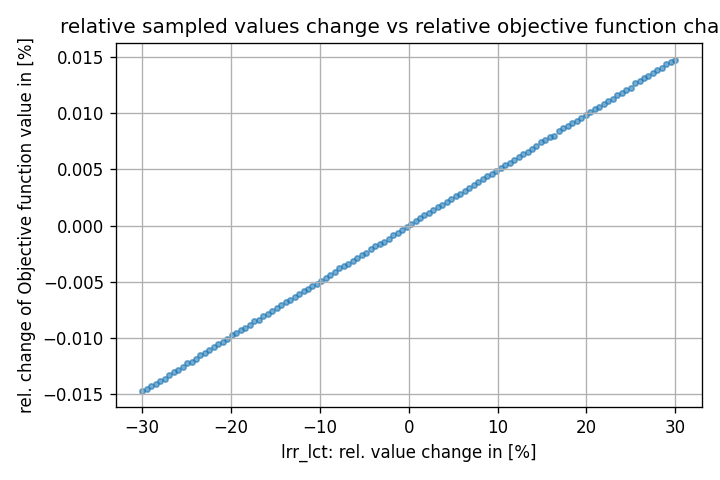
\includegraphics[width=\textwidth]{Figures/Ass_02/new/param_scatter_lrr_lct.png}
    \end{minipage}
    \caption{Sensitivity scatter plot for \texttt{lrr\_lct} (loss coefficient).}
    \label{fig:scatter_lrr_2}
\end{figure}

\vspace{0.5cm}
\noindent\textbf{Simulated discharge response}

To illustrate the practical effect of parameter perturbations on the hydrograph, figure~\ref{fig:diss_sl0fcy} shows the observed versus simulated discharge for the most sensitive parameter (\texttt{sl0\_fcy}) at $-30\%$ and $+30\%$ perturbation, and figure~\ref{fig:diss_snwpmf} shows the same for \texttt{snw\_pmf}. For reference, figure~\ref{fig:diss_urr_wsr} shows an insensitive parameter (\texttt{urr\_wsr}) where the simulated discharge is visually unchanged.

\begin{figure}[!ht]
    \centering
    \begin{minipage}[t]{0.45\textwidth}
        \centering
        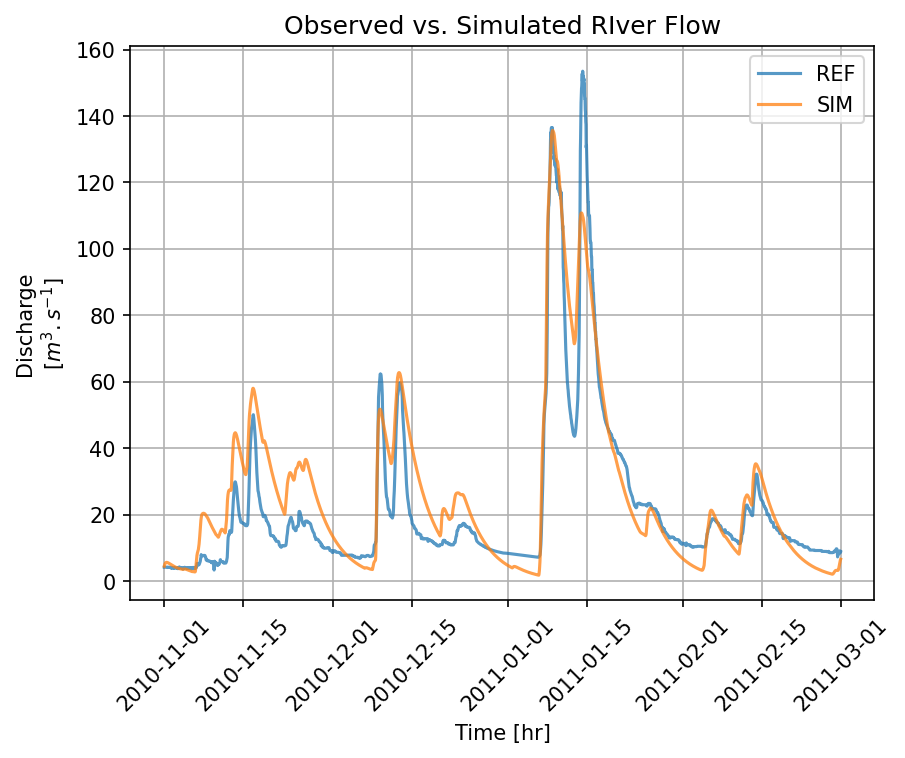
\includegraphics[width=\textwidth]{Figures/Ass_02/new/observed_vs_simulated_best_sl0_fcy_minus_30_percent.png}
    \end{minipage}
    \hfill
    \begin{minipage}[t]{0.45\textwidth}
        \centering
        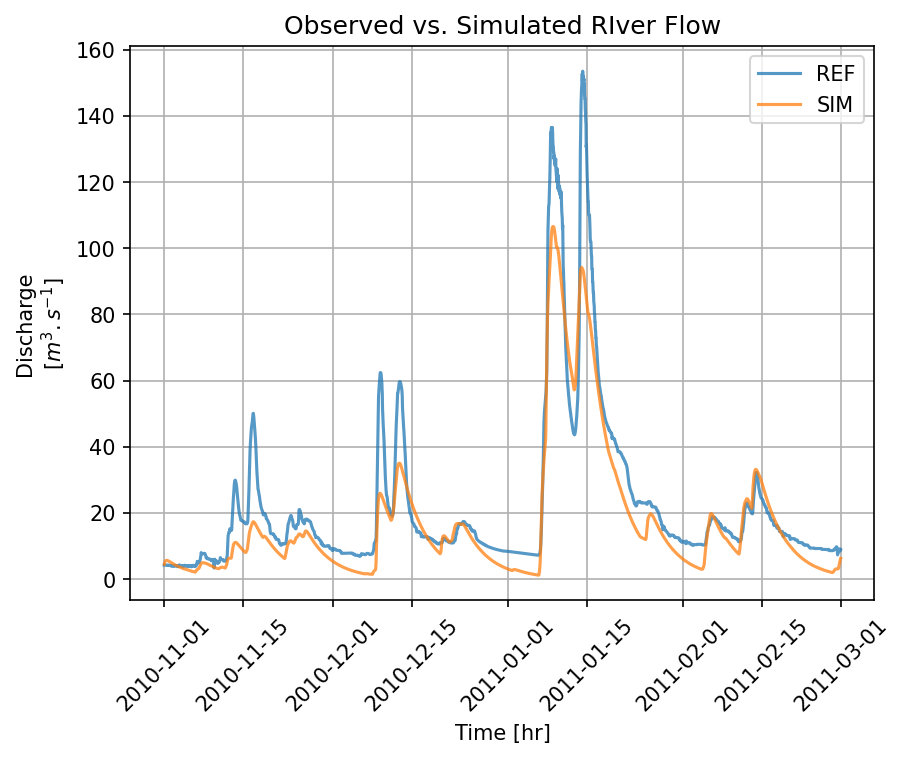
\includegraphics[width=\textwidth]{Figures/Ass_02/new/observed_vs_simulated_best_sl0_fcy_plus_30_percent.png}
    \end{minipage}
    \caption{Observed vs.\ simulated discharge for \texttt{sl0\_fcy} perturbed by $-30\%$ (left) generating more runoff and $+30\%$ (right).}
    \label{fig:diss_sl0fcy}
\end{figure}

\begin{figure}[!ht]
    \centering
    \begin{minipage}[t]{0.45\textwidth}
        \centering
        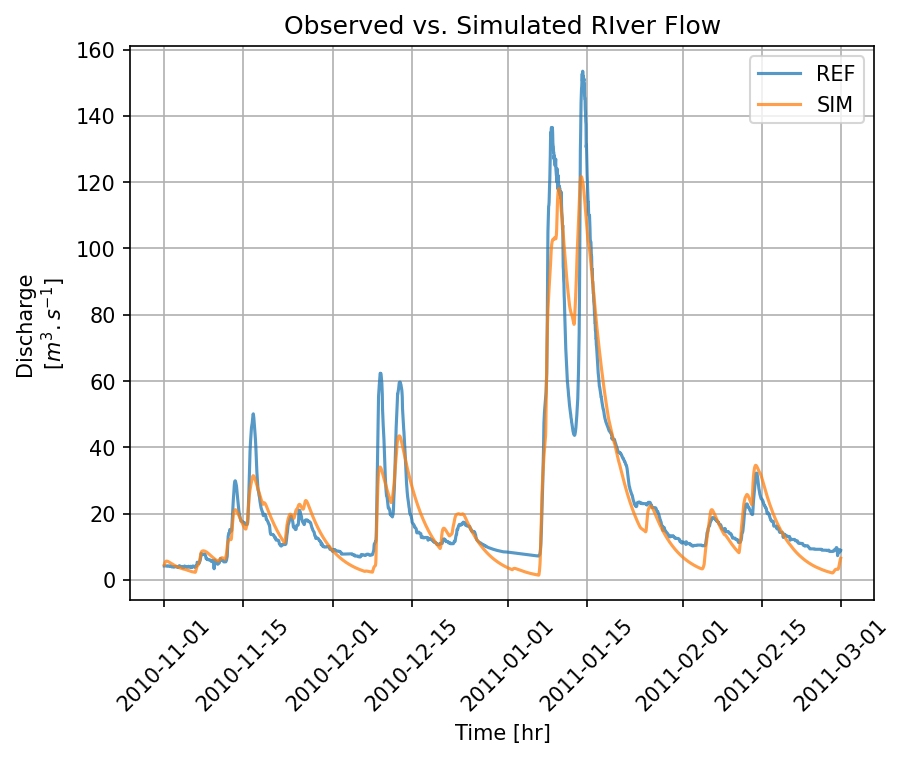
\includegraphics[width=\textwidth]{Figures/Ass_02/new/observed_vs_simulated_best_snw_pmf_minus_30_percent.png}
    \end{minipage}
    \hfill
    \begin{minipage}[t]{0.45\textwidth}
        \centering
        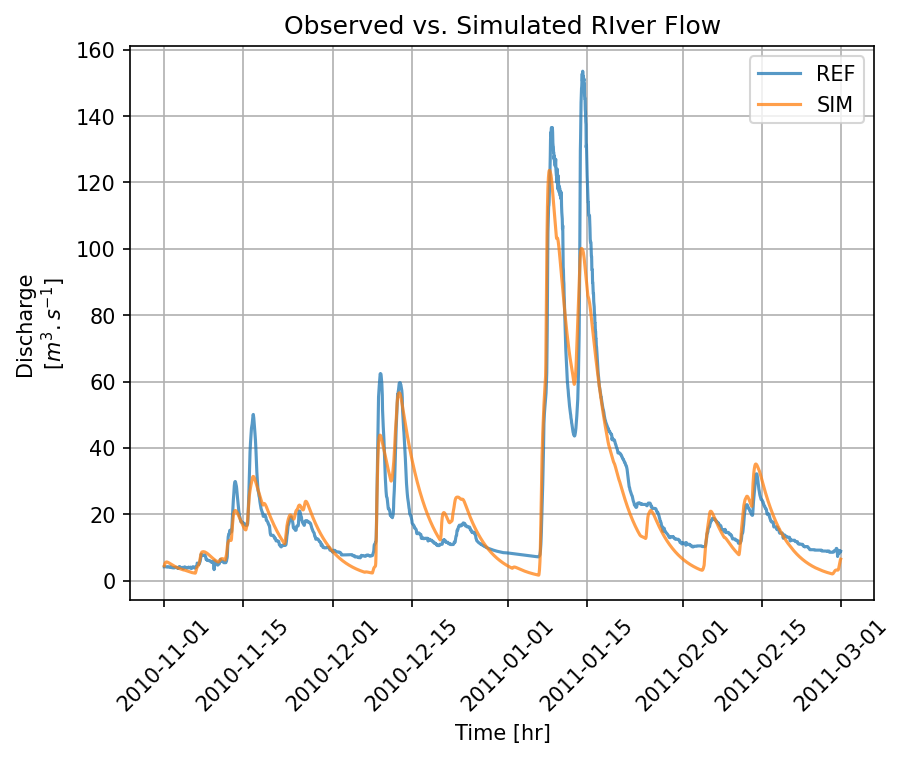
\includegraphics[width=\textwidth]{Figures/Ass_02/new/observed_vs_simulated_best_snw_pmf_plus_30_percent.png}
    \end{minipage}
    \caption{Observed vs.\ simulated discharge for \texttt{snw\_pmf} (precipitation melt factor) at $-30\%$ (left) and $+30\%$ (right). The influence of the snow melt is visible.}
    \label{fig:diss_snwpmf}
\end{figure}

\begin{figure}[!ht]
    \centering
    \begin{minipage}[t]{0.45\textwidth}
        \centering
        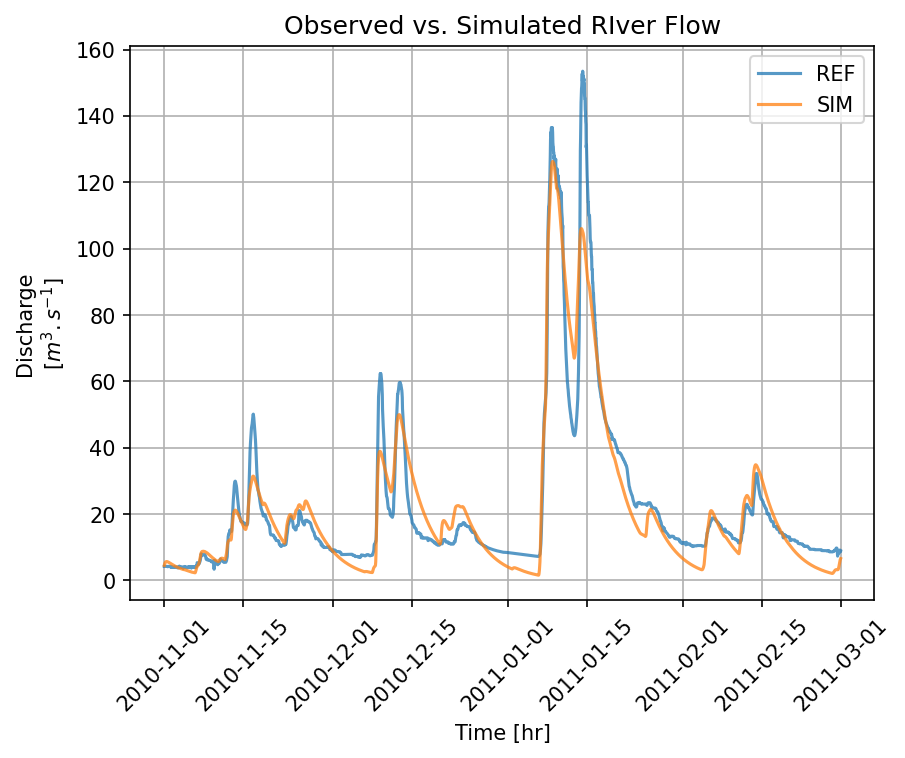
\includegraphics[width=\textwidth]{Figures/Ass_02/new/observed_vs_simulated_best_urr_wsr_minus_30_percent.png}
    \end{minipage}
    \hfill
    \begin{minipage}[t]{0.45\textwidth}
        \centering
        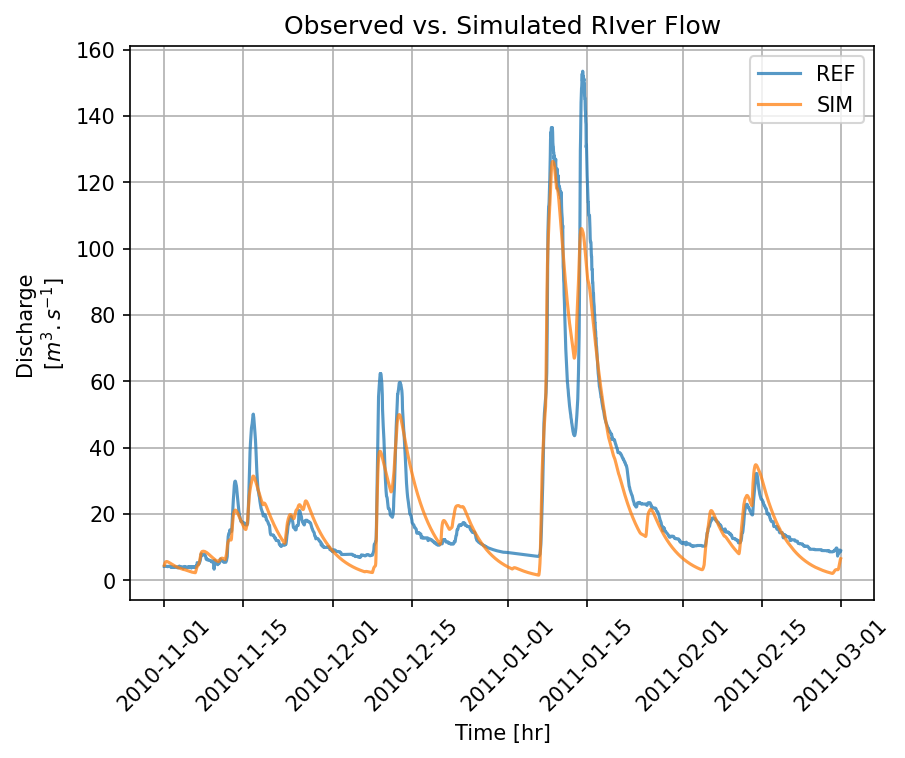
\includegraphics[width=\textwidth]{Figures/Ass_02/new/observed_vs_simulated_best_urr_wsr_plus_30_percent.png}
    \end{minipage}
    \caption{Observed vs.\ simulated discharge for \texttt{urr\_wsr} perturbed by $-30\%$ (left) and $+30\%$ (right). The effect is visual, not noticeable.}
    \label{fig:diss_urr_wsr}
\end{figure}



\vspace{0.5cm}
\noindent\textbf{Internal model state diagnostics}

Figure~\ref{fig:hbv_sl0fcy} shows the internally simulated HBV state variables for \texttt{sl0\_fcy} perturbed by $-30\%$ and $+30\%$. Comparing the two, the $-30\%$ case shows a clearly reduced soil moisture depth (SL0), and elevated surface runoff (RNF\,--\,SFC). In contrast, the $+30\%$ case shows a slightly deeper soil reservoir with marginally dampened runoff peaks, explaining the gradual degradation.

\begin{figure}[!ht]
    \centering
    \begin{minipage}[t]{0.45\textwidth}
        \centering
        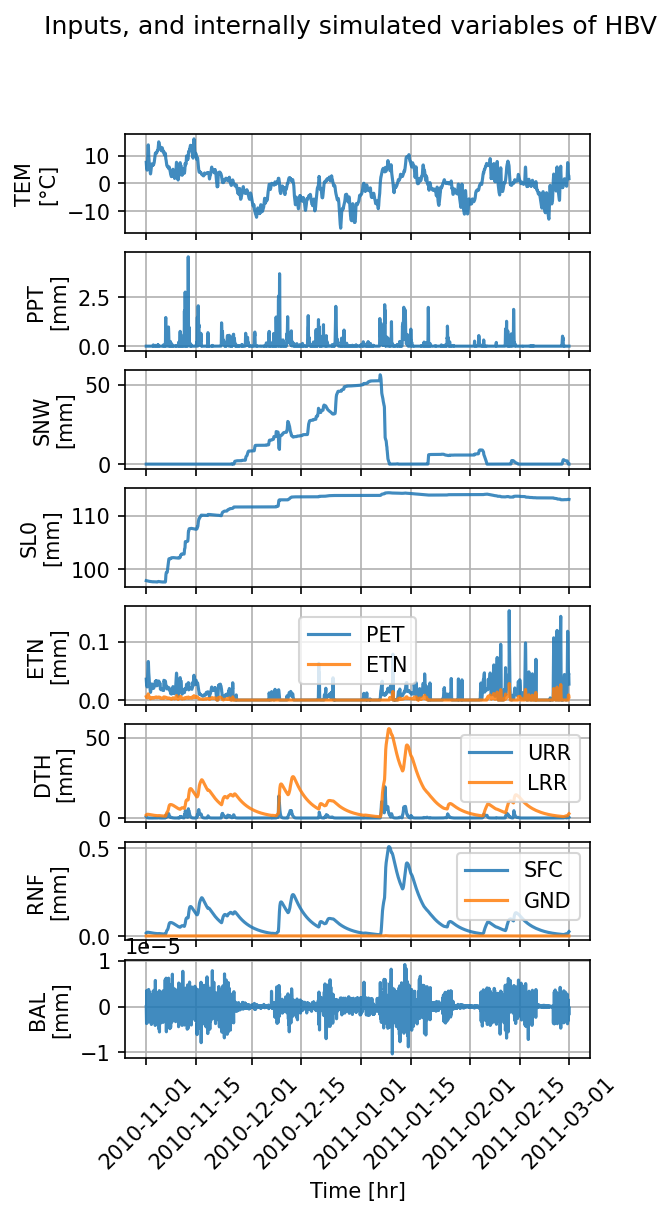
\includegraphics[width=\textwidth]{Figures/Ass_02/new/Inputs, and internally simulated variables of HBV sl0_fcy_minus_30_percent.png}
    \end{minipage}
    \hfill
    \begin{minipage}[t]{0.45\textwidth}
        \centering
        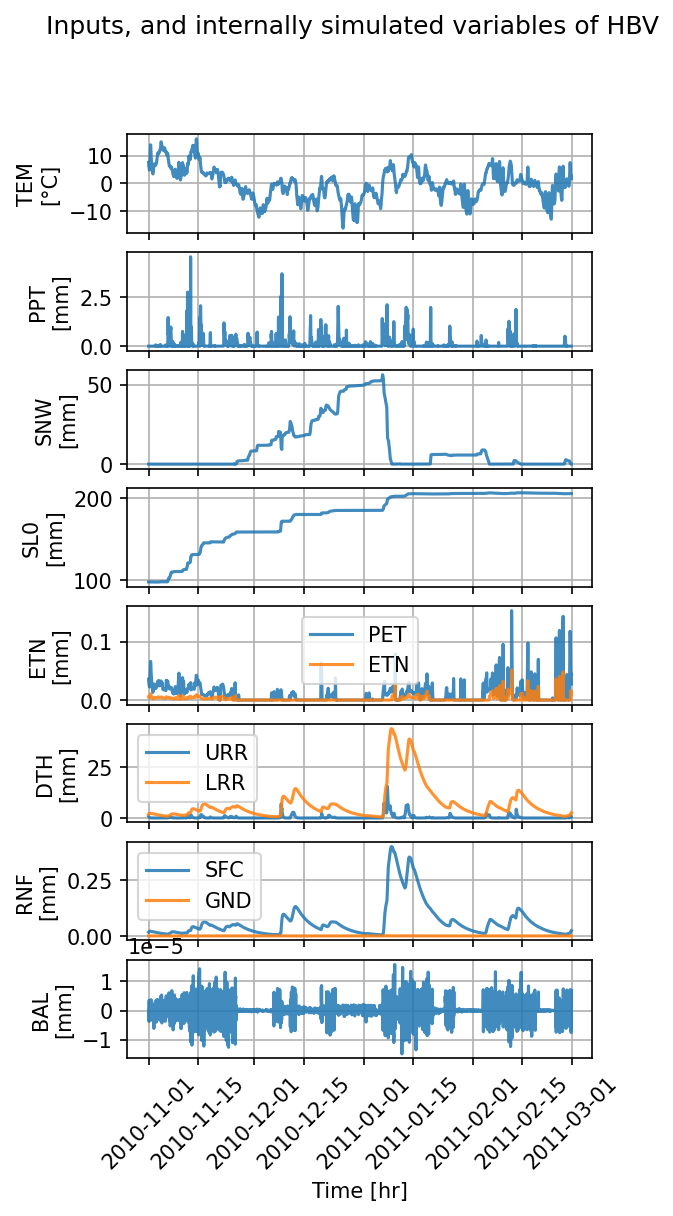
\includegraphics[width=\textwidth]{Figures/Ass_02/new/Inputs, and internally simulated variables of HBV sl0_fcy_plus_30_percent.png}
    \end{minipage}
    \caption{Internally simulated HBV state variables for \texttt{sl0\_fcy} at $-30\%$ (left) and $+30\%$ (right). From top to bottom: temperature (TEM), precipitation (PPT), snow depth (SNW), soil moisture (SL0), evapotranspiration (ETN), reservoir depths (DTH), runoff components (RNF), and water balance (BAL).}
    \label{fig:hbv_sl0fcy}
\end{figure}

\vspace{0.5cm}
\noindent\textbf{Summary}

The results emphasize that the soil module parameters, particularly \texttt{sl0\_fcy} and \texttt{sl0\_dth}, and the lower reservoir routing parameter \texttt{lrr\_dre}, are the dominant controls on model performance for this event. Snow-melt-related parameters are also relevant. The upper reservoir parameters play a negligible role due to a short calibration duration.

\vspace{0.5cm}
\noindent\textbf{Suggestions on how to have a non-sensitive (X)}

Based on the repository evidence, a parameter (X) becomes non-sensitive in the local One-At-a-Time sensitivity analysis through four main mechanisms, with one additional boundary-clamping effect that can mimic flatness.

First, (X) can be *structurally fixed at a boundary*. This occurs when the parameter has no effective freedom to vary. The clearest example is snw\_dth, whose calibrated value is 0.0 and whose bounds are also fixed at 0.0. Every perturbation is therefore clamped back to the same value, so the objective function remains unchanged. In this case, non-sensitivity is built directly into the model structure.

Second, (X) can become non-sensitive when the model process it controls is inactive. The example is snw\_att. Although this parameter has a genuine admissible range and is actually perturbed, its scatter plot remains perfectly flat. The reason is that $snw_dth = 0$ switches off the snow-related process, so changing snw\_att cannot influence the simulation. This shows that a parameter may be non-sensitive not because of its own numerical value, but because the sub-process it belongs to is inactive.

Third, (X) can appear non-sensitive when the calibrated solution lies in a locally flat region of the response surface. Around the optimum from Assignment 1, several parameters cause only very small changes in the objective function under ±30\% perturbations. In such cases, the local derivative of the objective with respect to (X) is close to zero, so the parameter looks non-sensitive in local sensitivity analysis. However, this can be misleading: Assignment 3 shows that some parameters that appear weak locally, such as urr\_ndr, are actually important in global sensitivity analysis. So this mechanism produces only apparent local non-sensitivity, not true global non-sensitivity.

Fourth, (X) can seem non-sensitive when its calibrated value is extremely small, so that even a relatively large percentage perturbation produces only a tiny absolute change. Parameters such as urr\_ndr, urr\_uct, and lrr\_lct fall into this category. Their local effect is small because the actual numerical variation remains tiny near the calibrated point. Again, this does not mean the parameter is truly unimportant over its full feasible range.

A further point is that boundary clamping can create flat-looking regions that should not be confused with true insensitivity. The example is sl0\_dth. Its right-side scatter plot is flat because many positive perturbations are clamped to the upper bound of 100.0. Since the input is frozen at that constant boundary value, the objective function also stays constant. It is a region of constant response caused by clamping, not genuine non-sensitivity.

\vspace{0.5cm}
\noindent\textbf{Conclusion}

The repository suggests that a non-sensitive (X) can be obtained most reliably in two ways:
by fixing (X) at a hard boundary, or by disabling the process that (X) controls.

The other cases — local flatness near the optimum and extremely small calibrated values — only make (X) appear non-sensitive in local analysis. They must be interpreted carefully, especially when checked against the global Sobol results. Also, flat segments caused by boundary clamping, such as for sl0\_dth, are not true insensitivity; they are artifacts of the perturbation hitting a fixed bound.

